\chapter{Планирование путей} \label{chapt1}


\section{Введение} \label{sect1_1}
Прежде чем робот сможет выполнить движение нужно знать, как и куда робот должен двигаться. Данную задачу разделяют на две составляющие: планирование пути и планирование траектории. Первая решает кинематическую задачу, определяя несколько дискретных точек, через которые должен пройти робот, чтобы избежать столкновения с препятствиями. Вторая - задачу динамики, на этом этапе составляются циклограммы движения с заданными начальными условиями и ограничениями на скорости и ускорения. Кроме того обе задачи можно также разделить на два подтипа: генерирование пути или траектории заранее или в режиме реального времени. Первый случай отлично подходит, если среда, в которой работает робот, статична, т.е. препятствия не меняют своего расположения. Второй подход решает проблему работы в изменяющейся во времени среде, но не обеспечивает какой либо оптимальности в планировании траекторий.

В ROS интегрирован фреймворк поиска путей и планирования траекторий \textbf{MoveIt}, который в свою очередь использует open source библиотеку \textbf{OMPL}, в которой реализованы все самые популярные sample based планировщики траекторий. Рассмотрим реализованные алгоритмы более подробно.

\section{Алгоритмы планирования пути} \label{sect1_2}
\subsection{Grid based search}\label{subsect1_2_1}
Одним из видов представления карты окружающей среды является разбиение карты на дискретную сетку. Для данного способа представления карты можно использовать обычный двумерный массив или же граф. Каждой ячейке или ребру ставится в соответствие вес, который характеризует "цену" перемещения согласно некоторой функции потерь. При этом ячейкам с препятствиями присваивается очень большой(маленький) вес, чтобы исключить столкновения в пути.

Имея построенную карту можно планировать путь, используя классические алгоритмы поиска кратчайшего пути на графе, такие как алгоритм Дейкстры, $A^{*}$, $D^{*}$ и т.п.

\subsection{PRM}\label{subsect1_2_2}
Probabilistic roadmaps(PRM) - эффективный вероятностный алгоритм поиска путей в известной местности. Принцип работы достаточно прост: он заполняет карту $N$ случайными сэмплами из пространства состояний. Каждый раз, сгенерировав новое случайное состояние, алгоритм пытается соединить новую вершину с $k$ ближайшими соседями в графе или со всеми вершинами в некой окрестности $\delta$, проверяя при этом выполнение ограничений, наложенных динамикой системы, а также на столкновения. После того, как карта сгенерирована, можно планировать траектории. По уже описанному алгоритму к графу добавляются две новые вершины: исходная и целевая. После чего применяются стандартные алгоритмы поиска кратчайшего пути на графе, такие как алгоритм Дейкстры\cite{CLRS}, $A^{*}$\cite{AStarWiki} и т.п.

Из преимуществ алгоритма можно указать возможность повторного использования карт для разных начальных и конечных состояний, а также скорость работы после построения карты.

К недостаткам относятся экспоненциальный рост размера карты в зависимости от размерности пространства состояний, а также отсутствие оптимальности найденного пути во всех смыслах. Кроме того вероятность успешного поиска пути сильно зависит количества сэмплов $N$ и их распределения. Посмотрите на следующий рисунок:

\begin{figure}[ht]
    \centering
    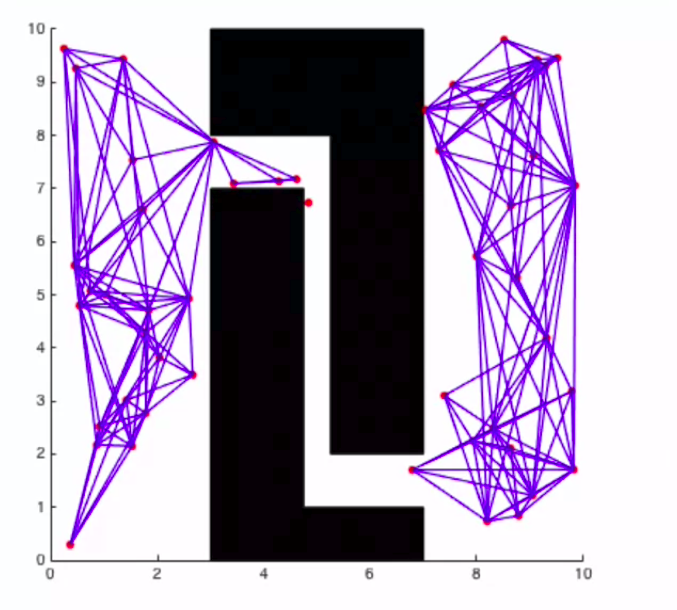
\includegraphics[scale=0.3]{PathPlanning/prm_stuck}
    \caption{Probabilistic road map не сможет найти путь}
\end{figure}

Проход между препятствиями слишком узок для того, чтобы в него попало достаточное количество сэмплов для построения пути. Эту проблему можно решить, выбирая сэмплы так, чтобы в окрестностях препятствий плотность их распределения была выше. Но это решение одной частной проблемы. На данный момент не существует универсального метода распределения случайных состояний на карте так, чтобы путь был найден при произвольной конфигурации окружающей среды.\cite{CourseraMotionPlanning}

\subsection{RRTConnect} \label{subsect1_2_3}
Одним из самых эффективных алгоритмов поиска пути является \textbf{RRTConnect}, который основан на использовании двух \textbf{RRT}(Rapidly-exploring random trees)\cite{RRTWiki}. Является probabilistically complete, в том смысле, что вероятность верно найденного решения стремится к единице, если время поиска $t \rightarrow \infty$.

Что же такое RRT? Это обычное дерево, к которому на каждой итерации построения добавляется случайная вершина. Чтобы построить данное дерево нужно определить два параметра: $\delta$, который определяет расстояние между вершинами дерева в пространстве поиска, и $N$ - максимальное количество итераций.

Допустим, на текущем шаге построения мы имеем следующее дерево:
\begin{figure}[ht]
    \centering
    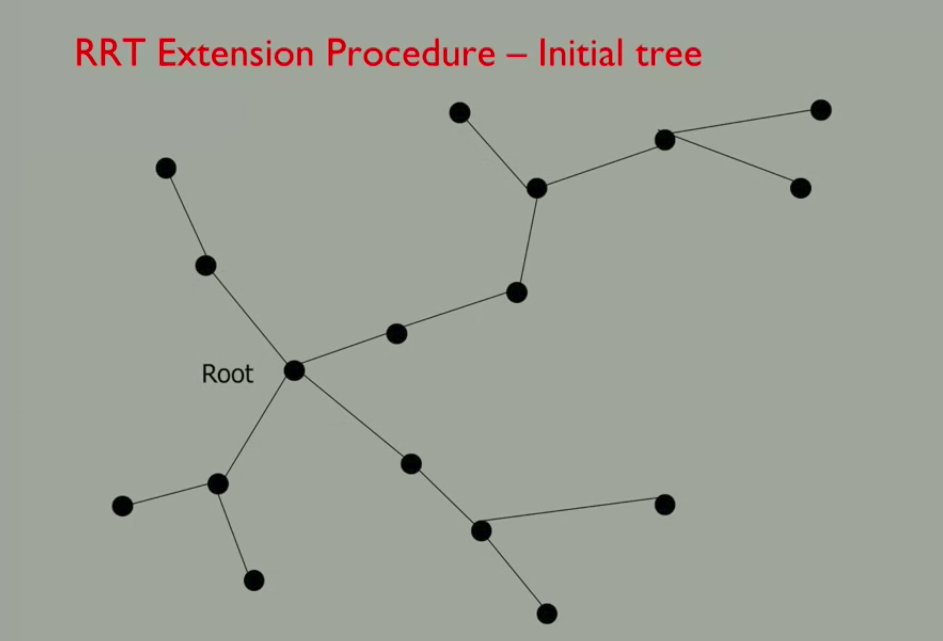
\includegraphics[scale=0.3]{PathPlanning/rrt_build_initial}
    \caption{Исходное дерево}
\end{figure}

Сначала случайным образом выбирается новая точка $X$ в пространстве поиска:
\begin{figure}[ht]
    \centering
    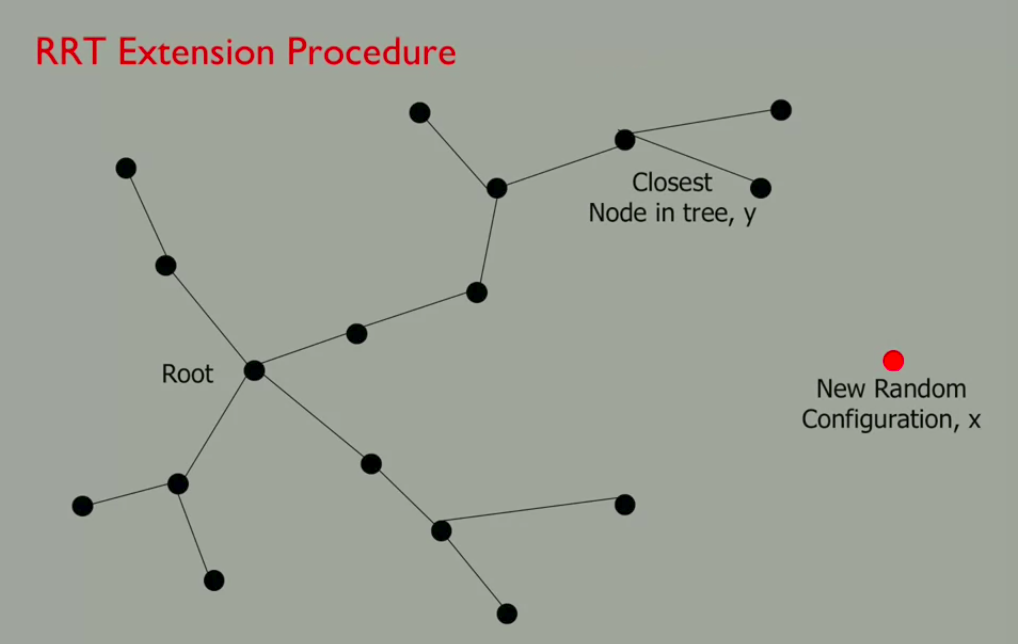
\includegraphics[scale=0.3]{PathPlanning/rrt_build_new_state}
    \caption{Новая случайная точка}
\end{figure}

После в дереве определяется ближайшая к ней вершина $Y$ и, если она находится на расстоянии меньшем чем $\delta$ от $X$, удовлетворяет всем ограничениям наложенными динамикой системы, а также на пути нет препятствий, то она добавляется к дереву. Если же вершина удалена больше, чем на $\delta$, то ее заменяют вершиной на расстоянии $\delta$ от вершины $Y$ на прямой, соединяющей ее с вершиной $X$. В случае, если путь не удовлетворяет ограничениям динамики, переходим к следующей итерации.
\begin{figure}[ht]
    \centering
    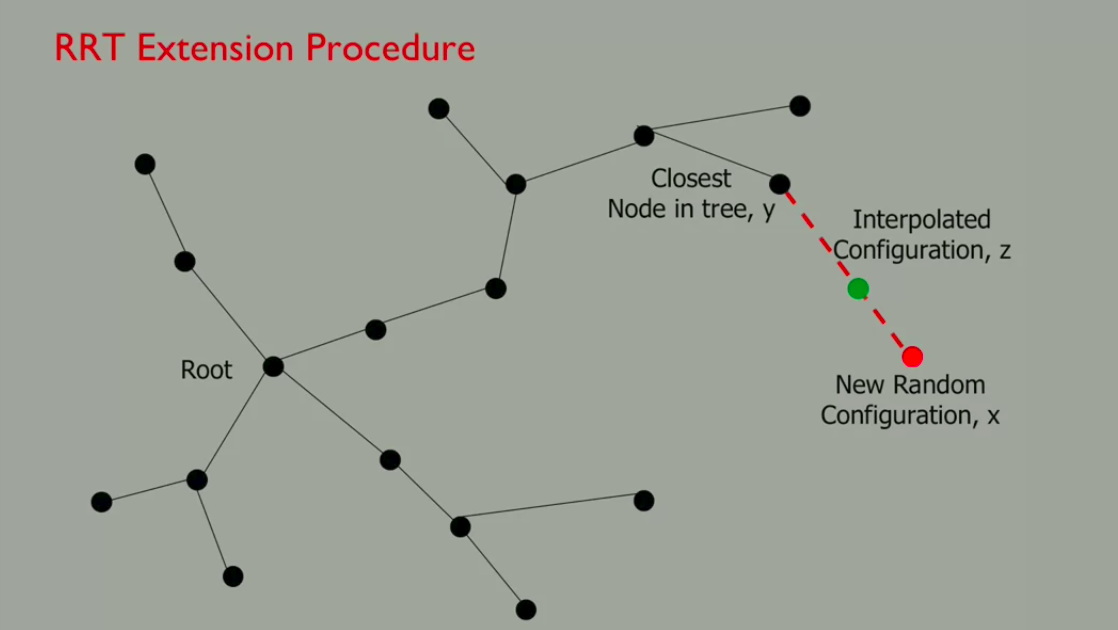
\includegraphics[scale=0.3]{PathPlanning/rrt_build_new_vertex}
    \caption{Добавляем новую вершину к дереву}
\end{figure}

RRTConnect строит два RRT дерева: одно - из текущей вершины, второе - из требуемого положения - и на каждой итерации пытается соединить оба дерева. В алгоритме построения есть одно небольшое изменение - операция extend для вершины $X$ выполняется до тех пор, пока на пути не возникнет препятствия или эта вершина не окажется добавленной к дереву. Путь считается найденным, если оба дерева оказались соединены. Если же количество итераций превысило $N$, поиск считается проваленным.\cite{RRTConnect}

Преимуществами данного алгоритма является крайне высокая практическая эффективность.\cite{RRTConnect} Поэтому он является одним из самых популярных алгоритмов поиска пути. К недостатками относится отсутствие оптимальности найденного пути.

\section{Сглаживание путей}\label{sect1_3}
